\documentclass[titlepage]{article}
    \title{\textbf{AI Project 3 Report}}
    \author{Tobias Dault, Eyob Tekle, William Thomson Jr.}
    \date{1 April 2022}
    
    \addtolength{\topmargin}{-3cm}
    \addtolength{\textheight}{3cm}
\usepackage{graphicx}
\usepackage{hyperref}
\graphicspath{ {./assets/} }

\begin{document}
\maketitle
\tableofcontents
\newpage
\thispagestyle{empty}

\section{Introduction}
The purpose of our program is to collect names of attributes, values of attributes, hard constraints, and preferences for the reason of performing four reasoning tasks: Existence of feasible objects, exemplification, optimization, and omni-optimization.
\newpage

\section{Input}
Using a GUI written in Python (using Tkinter framework), input is taken through either the text input boxes or file input buttons.

\addtolength{\itemindent}{0.80cm}
\itemsep0em
\subsection{Binary Attributes}
Step 1: Follow steps in the README to start the program\\
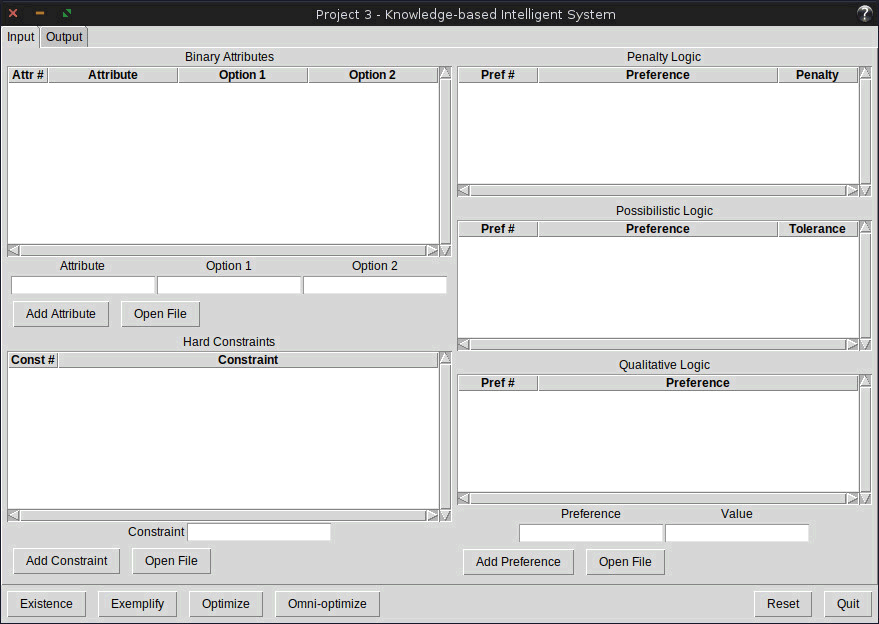
\includegraphics[scale=0.3]{input_start} \\\\
Step 2: Click the "Open File" button under Binary Attributes\\
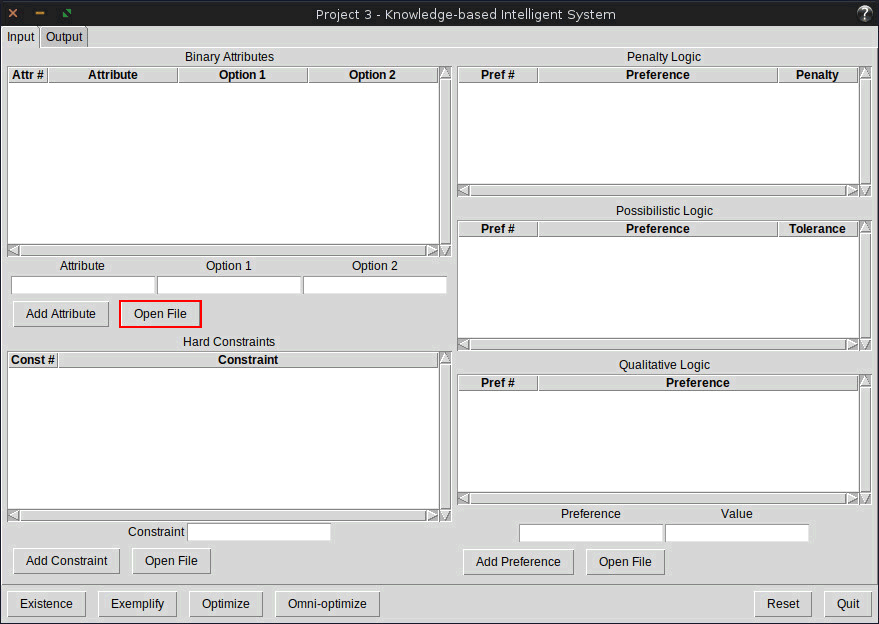
\includegraphics[scale=0.3]{input_attributes}\newpage
Step 3: Select your desired file (attributes$\_$test.txt for this example) and click "Open".\\
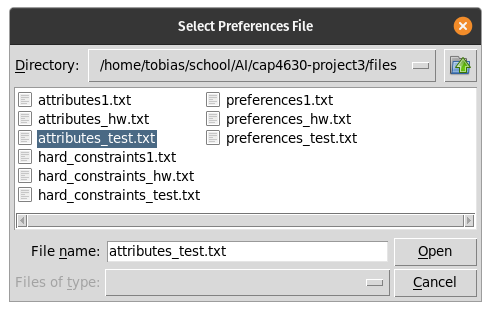
\includegraphics[scale=0.3]{select_attributes}\\
The contents of the file will be displayed under Binary Attributes.\\
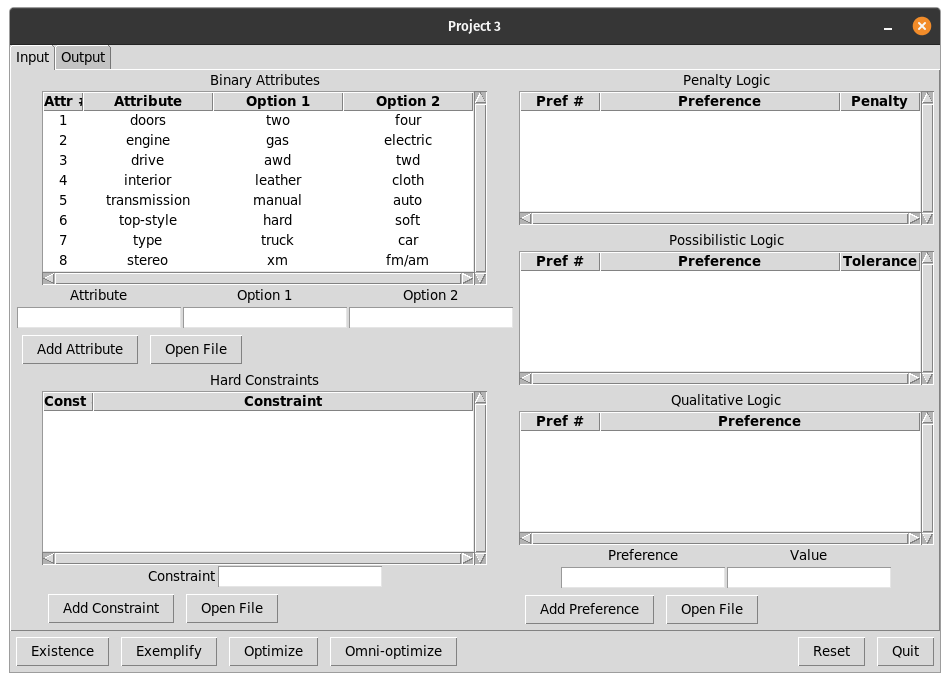
\includegraphics[scale=0.3]{attributes_imported}
\newpage

\subsection{Hard Constraints}
Step 1: Click the "Open File" button under Hard Constraints\\
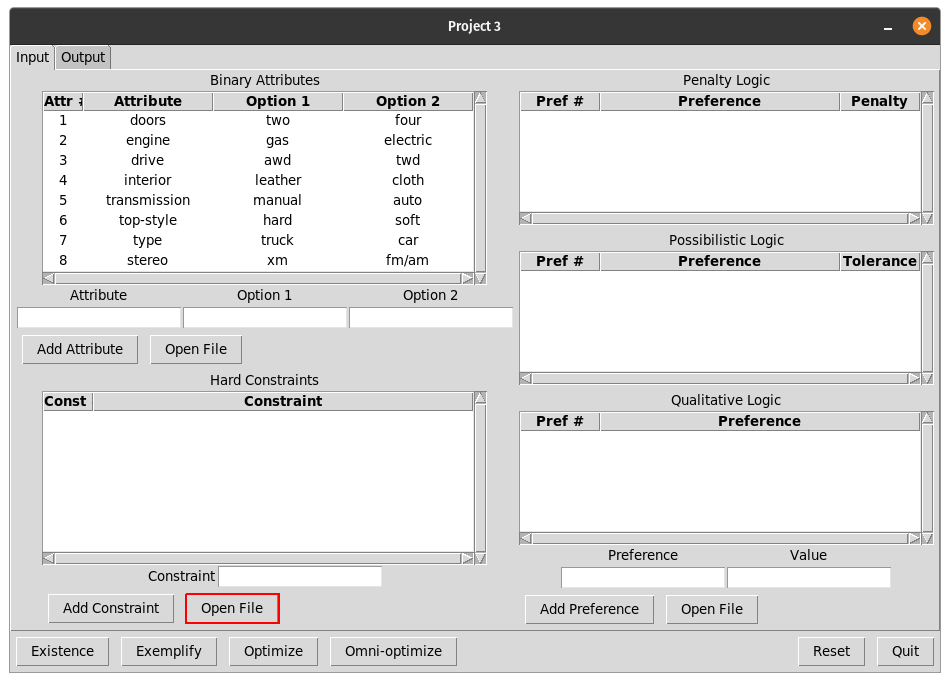
\includegraphics[scale=0.3]{input_constraints} \\\\
Step 2: Select your desired file (hard$\_$constraints$\_$test.txt for this example) and click "Open".\\
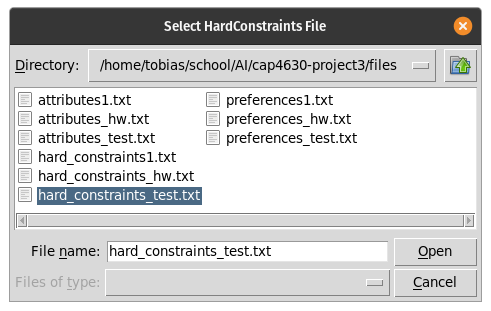
\includegraphics[scale=0.3]{select_constraints}\\
Step 3: The contents of the file will be displayed under Hard Constraints.\\
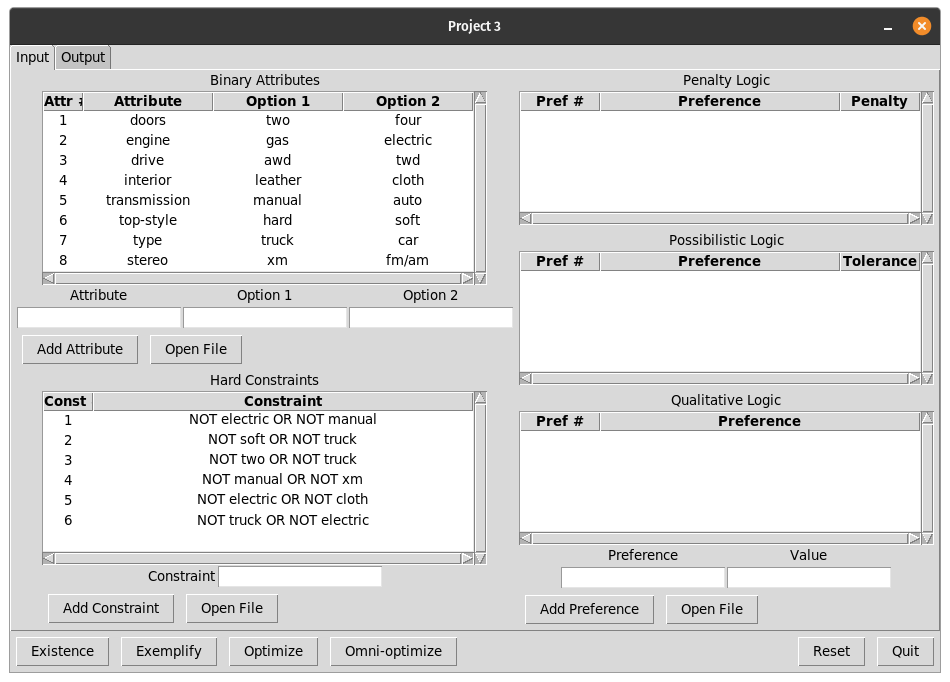
\includegraphics[scale=0.3]{constraints_imported}\\

\subsection{Logics}
Step 1: Click the "Open File" button under the three logics\\
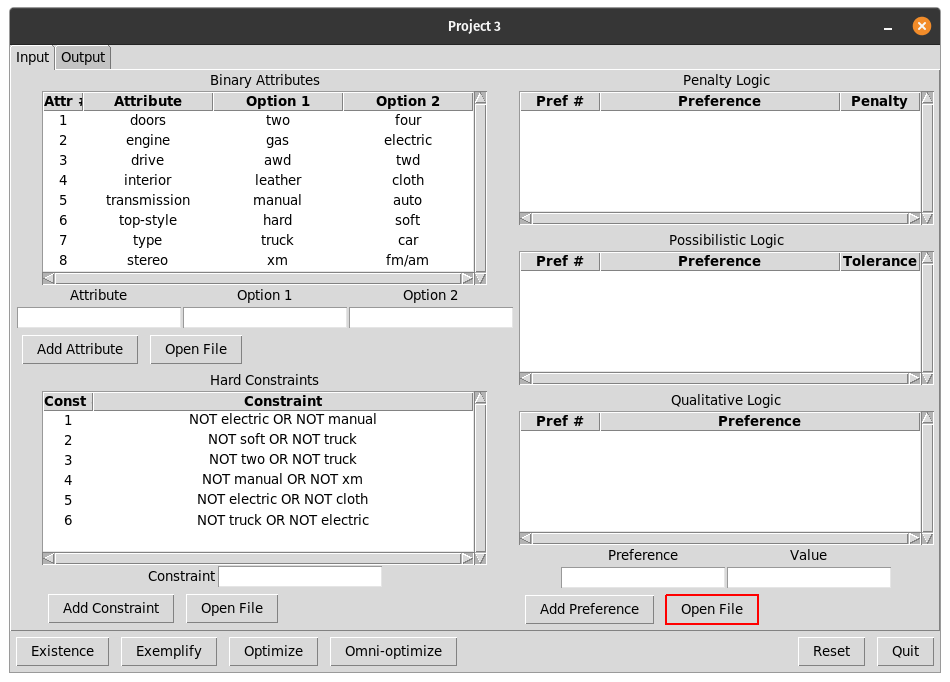
\includegraphics[scale=0.3]{input_preferences} \\\\
Step 2: Select your desired file (preferences$\_$test.txt for this example) and click "Open".\\
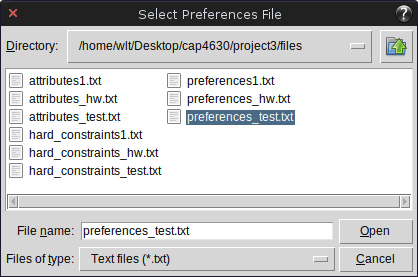
\includegraphics[scale=0.3]{select_preferences}\\
Step 3: The contents of the file will be displayed in the three.\\
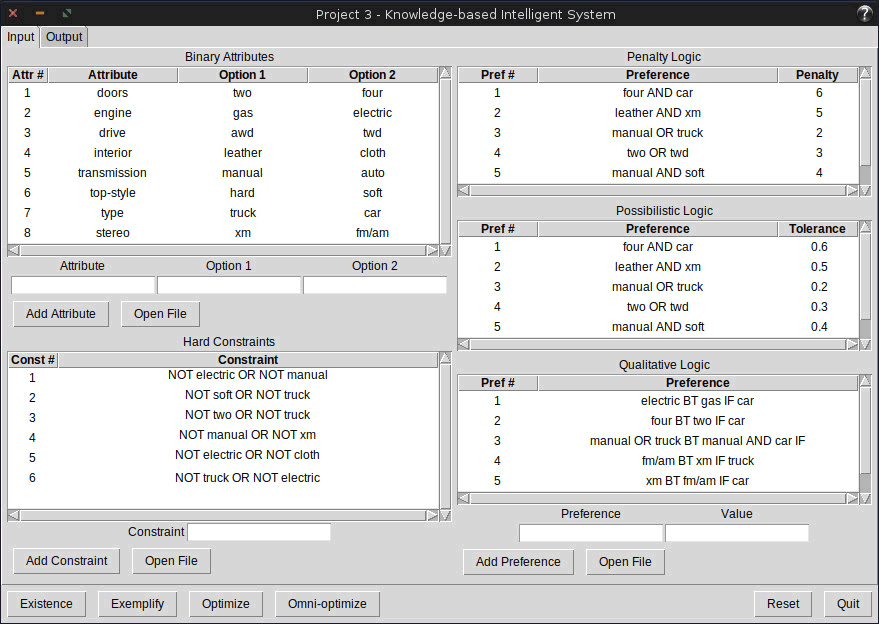
\includegraphics[scale=0.3]{preferences_imported}
\newpage

\section{Output}
\subsection{Existence of Feasible Objects} Click the "Existence" button\\
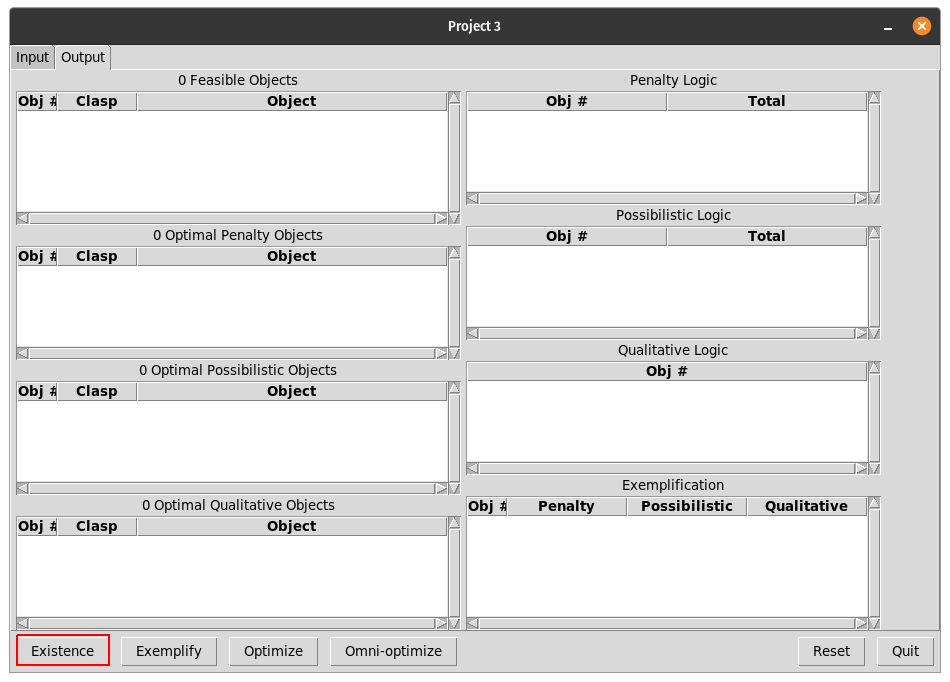
\includegraphics[scale=0.3]{existence}\\
All feasible objects, as well as a count of the total number of them, have been generated inside the "Feasible Objects" window.\\
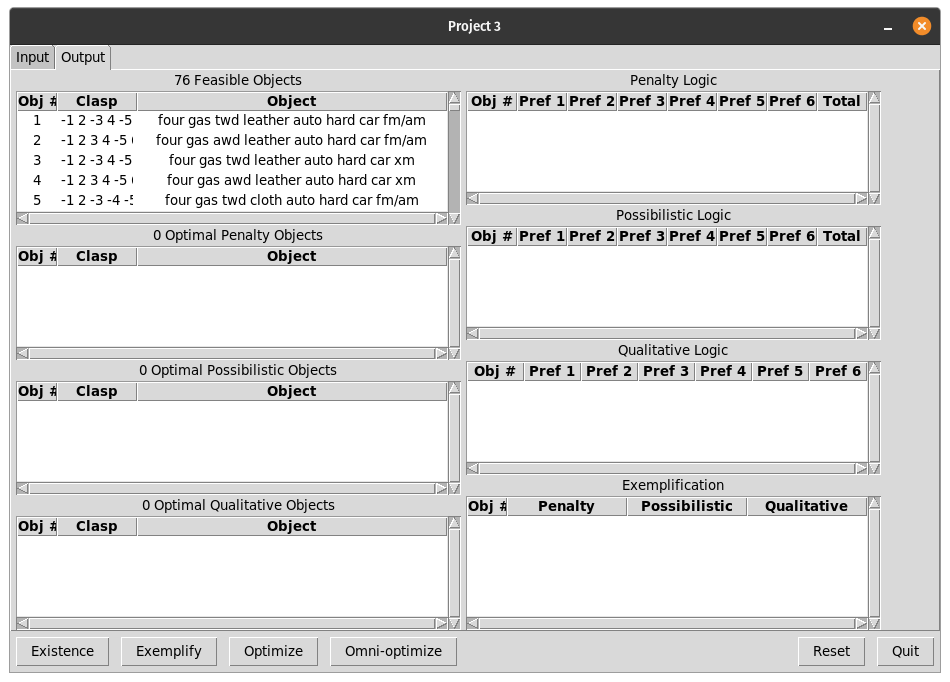
\includegraphics[scale=0.3]{post_existence}
\newpage

\subsection{Exemplify} Click the "Exemplify" button\\
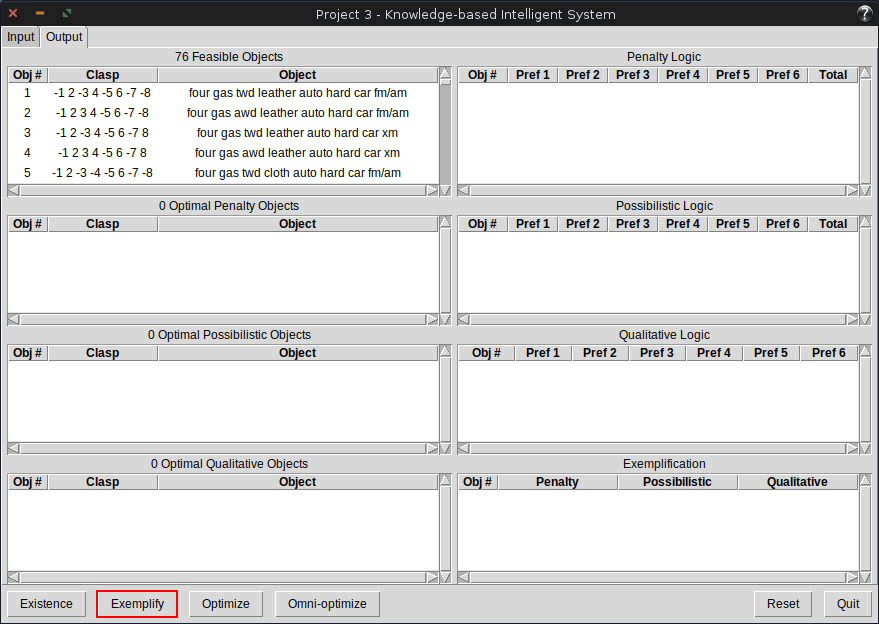
\includegraphics[scale=0.3]{exemplify}\\
The Penalty, Possiblistic, and Qualitative Logic tables have been generated. The exemplification table shows which objects are prefered for each logic.\\
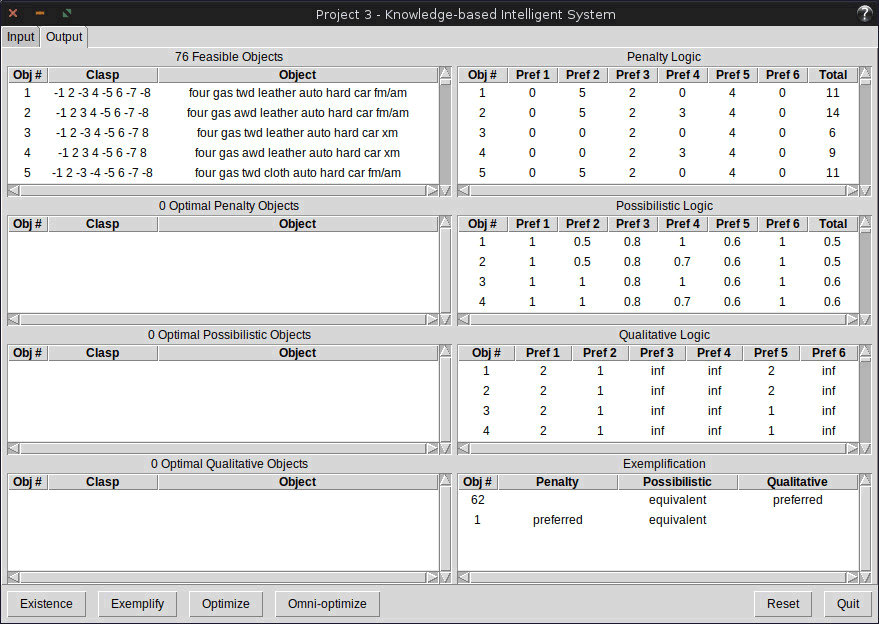
\includegraphics[scale=0.3]{post_exemplify}
\newpage

\subsection{Optimize} Click the "Optimize" button\\
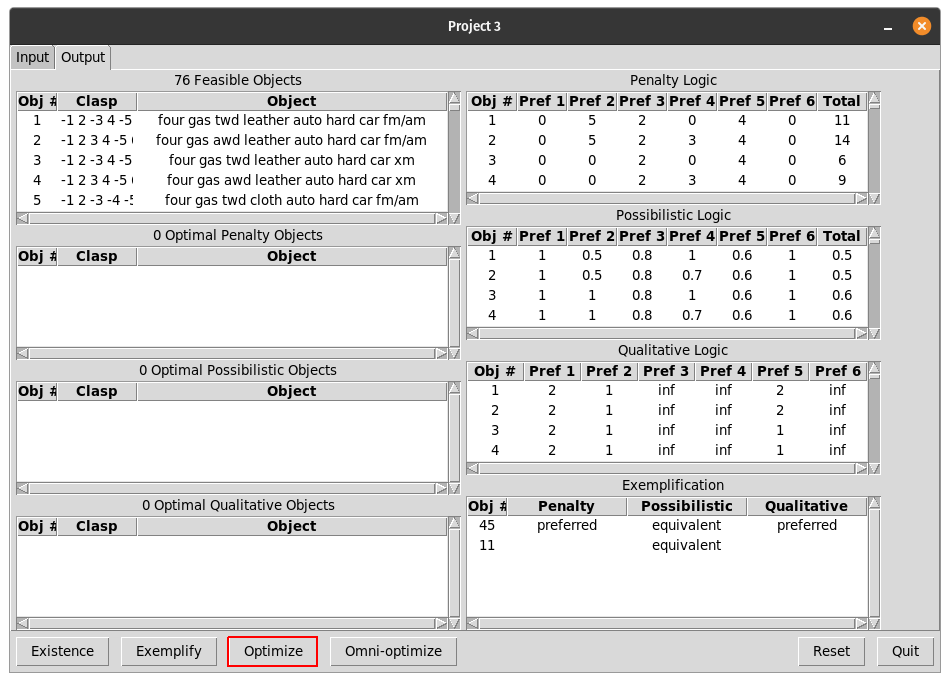
\includegraphics[scale=0.3]{optimize}\\
The Penalty, Possiblistic, and Qualitative Logic tables have been generated. The exemplification table shows which objects are prefered for each logic.\\
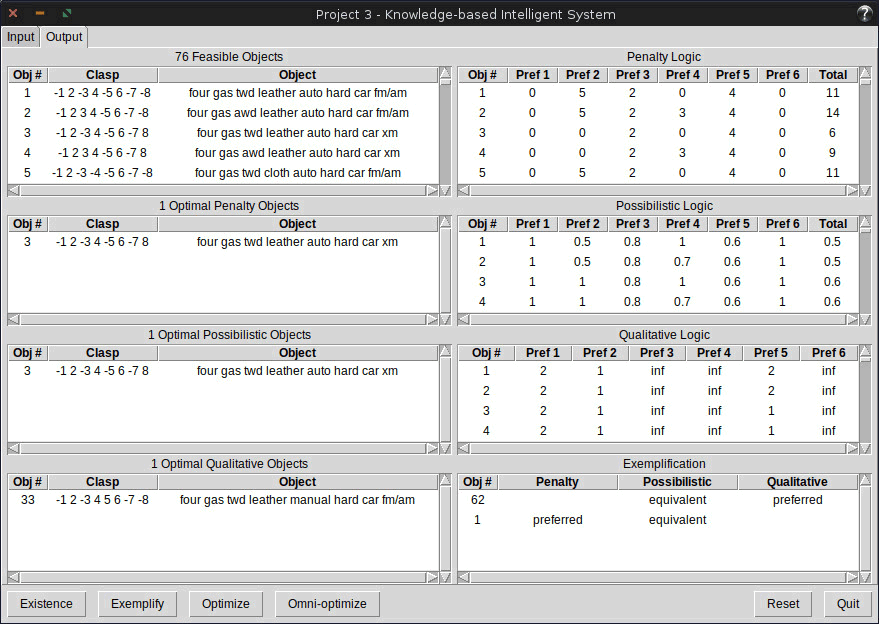
\includegraphics[scale=0.3]{post_optimize}
\newpage

\subsection{Omni-optimize} Click the "Omni-optimize" button\\
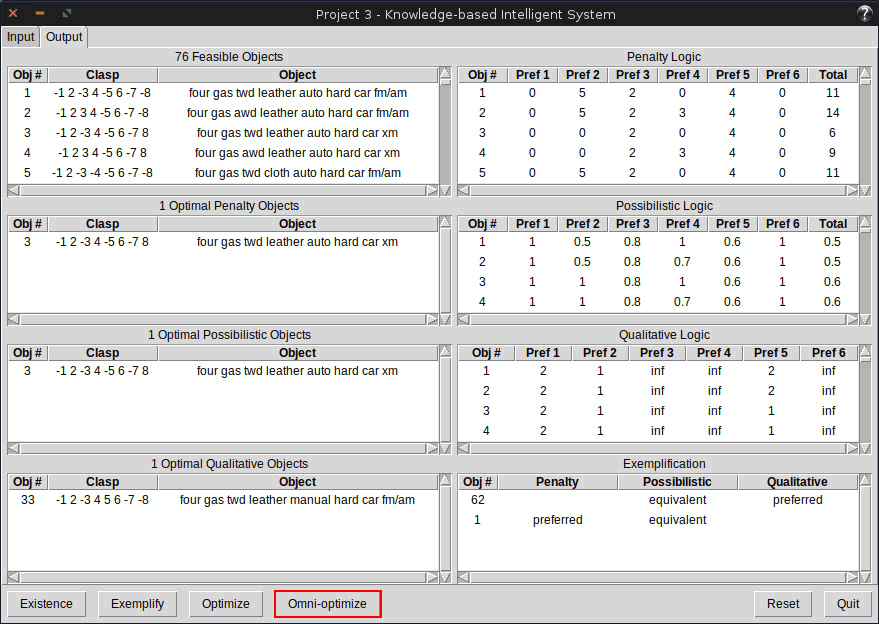
\includegraphics[scale=0.3]{omni-optimize}\\
The Penalty, Possiblistic, and Qualitative Logic tables have been generated. The exemplification table shows which objects are prefered for each logic.\\
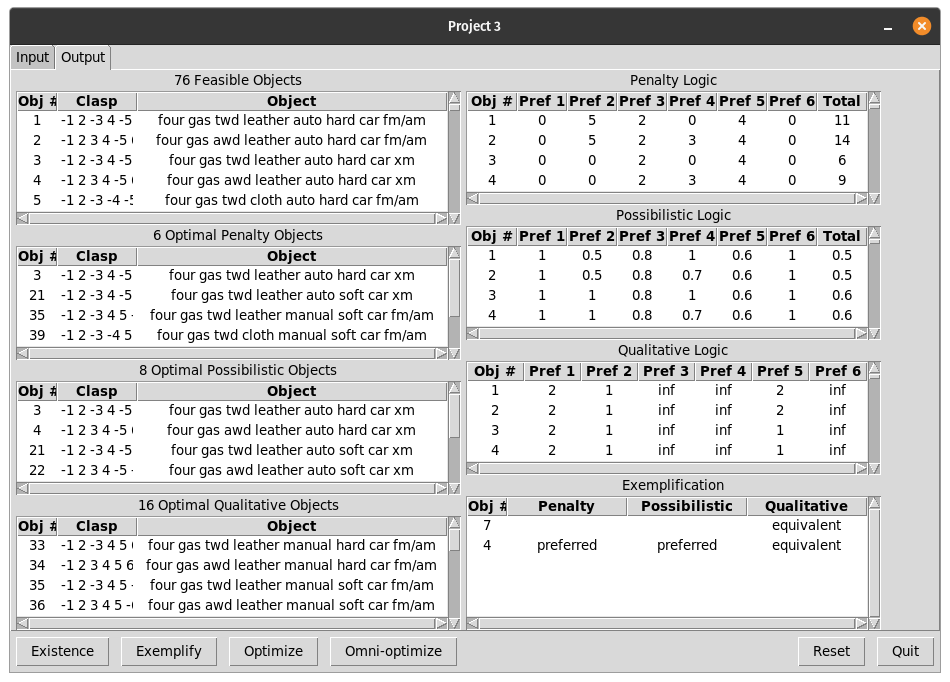
\includegraphics[scale=0.3]{post_omni-optimize}


\end{document}